%!TEX root = ../thesis.tex
% Spellcheck ignore
% cSpell:ignore realrubidium, giga, levelscheme, deexcite, eqref, weakfield, intlorgau, gauvslor, atomicmassunit, citep, ifpdf, graphicspath, bigskip, minipage, includegraphics, twolevel, captionof, nano, FWHM, linewidth, electronvolt, Linewidth, nlinewidth, Lorentzian, pagebreak, wrapfigure, photodiode, mathrm, itemsep, extracolsep, toprule, multicolumn, midrule, bottomrule, energylevel, hyperfine, groundstate, nist, groundstates, nonumber, Lorentzians
%*******************************************************************************
%****************************** Second Chapter *********************************
%*******************************************************************************

\ifpdf{}
\graphicspath{{Chapter2/Figs/Raster/}{Chapter2/Figs/PDF/}{Chapter2/Figs/}}
\else
\graphicspath{{Chapter2/Figs/Vector/}{Chapter2/Figs/}}
\fi

\chapter{Absorption of photon by an atom}  %Title of the Second Chapter
The purpose of this section is to outline the basic features observed in 
saturated absorption spectroscopy and relate them to simple atomic and laser 
physics principles. For this we will follow the guidance of \citep{SAS} and 
\citep{SAS_appendix}.

Electrons can orbit around the atom nucleus following different trajectories which
are quantified, the so called orbitals. It is energetically preferable that the
electron orbit around the atomic nucleus in the lowest possible orbitals, but it 
is possible to excite the electron in different higher excited states. The 
difference of energy states are in the range of typically optical frequencies, 
which give rise to absorption spectrum. The atomic transitions are sufficiently 
separated such that, when probing close to one resonance, one can consider that 
they behave as a 2 level system.

%********************************** % First Section  *************************************
\section{Laser interactions~-~Two-level atom} %Section - 2.1

We begin with the interaction between a laser field and a sample of stationary 
atoms having only two possible energy levels. Aspects of thermal motion will 
be treated subsequently.\\ 
The ground state is denoted \ket{g} of energy \(E_0 \) and the excited state 
\ket{e} of energy \(E_1 \). The transition frequency \(\nu_0 \) is given by 
Planck's law
\begin{align}
    h \nu_0 = E_1 - E_0~.
\end{align}
For the considered transition, \(\nu_0 \) is in the optical domain.
There can three transition processes happen, as described in Fig.~\ref{fig:twolevel}:
\pagebreak

\begin{figure}[h]
    \centering
    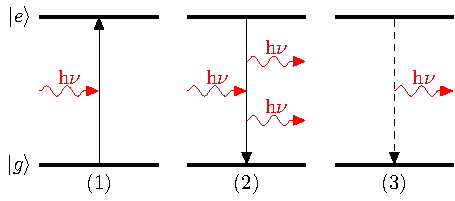
\includegraphics[width=0.6\textwidth]{twolevel}
    \caption{\label{fig:twolevel}Two-level atom model}
\end{figure}


\begin{itemize}
\item[(1)] \textit{absorption}: Atom in the ground state absorbs a photon with 
    the energy \(h \nu_0 \) and is excited. The absorption process is described
    by a transition rate or probability per unit time and is proportional to the
    laser intensity \textit{I} (SI units of \si{\watt\per\meter\squared}) and is
    only significantly different from zero when the laser frequency \(\nu \) is
    near the resonance frequency \(\nu_0 \) of the transition. This transition
    rate will be denoted \(\alpha~I \), where

    \bigskip
    \begin{minipage}[c][][c]{.45\textwidth}
        \begin{align}\label{eq:alpha}
            \alpha = \alpha_0~\mathcal{L}(\nu,\nu_0)
        \end{align}
        and
        \begin{align}
            \mathcal{L}(\nu,\nu_0) &= \frac{1}{ 1+4~{(\nu-\nu_0)}^2 / {\Gamma_\nu}^2 }
        \end{align}
    \end{minipage}
    \hfill
    \begin{minipage}[c]{.45\textwidth}
        \centering
        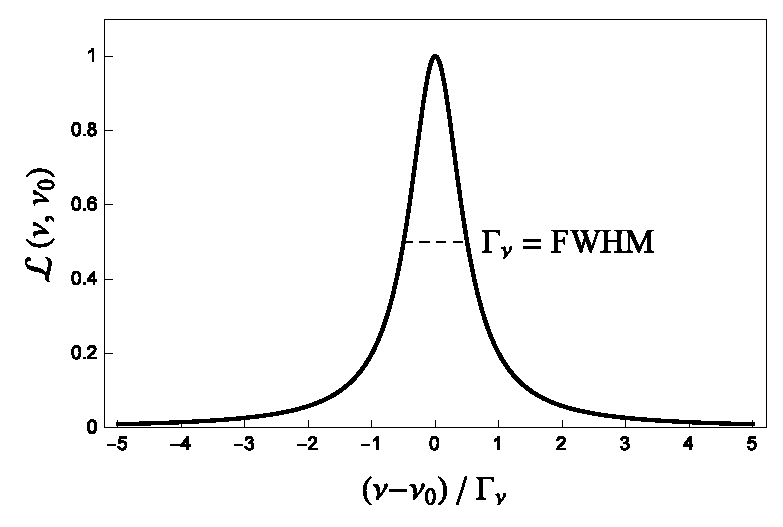
\includegraphics[width=.9\textwidth]{nLinewidth}
        \captionof{figure}{\label{fig:nlinewidth} The Lorentzian line shape profile 
            for a transition}
    \end{minipage}

    \bigskip
    gives the \textit{Lorentzian} frequency dependence with a full width at half
    maximum (FWHM) or \textit{natural linewidth} \(\Gamma_\nu \) of this transition 
    as shown in Fig.~\ref{fig:nlinewidth}. The maximum transition rate \(\alpha_0~I \) 
    occurs right on resonance (\(\nu=\nu_0 \)).

    Another important value is 
    \begin{align}
        I_s = \frac{\Gamma_\omega}{\alpha_0} \label{eq:saturationInt}
    \end{align}
    which defines the saturation intensity of an atom and a specific state. Its 
    significance is that when the laser intensity is equal to the saturation intensity, 
    excited state atoms are equally likely to decay by stimulated emission or by 
    spontaneous emission.
\item[(2)] \textit{spontaneous emission}: In the absence of an external field,
    any initial population of excited state atoms will decay exponentially to the 
    ground state with a mean lifetime \(\Delta t\).
    In the rest frame of the atom, spontaneous photons are emitted in arbitrary 
    directions and polarization with an energy spectrum having a mean \( E = h \nu_0 \) 
    and a FWHM \(\Delta E \) given by the Heisenberg uncertainty principle
    \(\Delta E~\Delta t = \hbar \) or \(\Delta E = \Gamma_\omega \hbar \) with 
    the transition rate \(\Gamma_\omega = \frac{1}{\Delta t}\). The transition 
    rate corresponds to the \textit{natural linewidth} of the transition
    \begin{align}\label{eq:gamma_relation}
        \Gamma_{\nu} = \frac{\Gamma_\omega}{2\pi}
    \end{align}
\item[(3)] \textit{stimulated emission}: If a photon of \(h\nu_0 \) impinges on
    an atom in the excited state, the atom will de-excite by emitting a photon
    which has the same characteristics (\(\vec{k}\), phase, polarization) as the
    incident photon. The process of stimulated emission is also described by the
    same transition rate \(\alpha~I \) as absorption, because the photon emitted
    or absorbed corresponds to the same transition line.
\end{itemize}


%********************************** % Second Section  *************************************
\section{The \(5S_{1/2}\rightarrow 6P_{3/2}\) transition of \(^{85}\)Rb}   %Section - 2.2

We want to probe the \(5S_{1/2}\rightarrow 6P_{3/2}\) transition, which is not
the lowest energy transition. Thus when the atom is in the \(6P_{3/2} \) state
it has several decay channels 
(e.g. \(6P_{3/2}\rightarrow 6S_{1/2} \rightarrow 5P_{3/2} \rightarrow 5S_{1/2}\)). 
Therefore the lifetime of the state 
\(\Delta t=\SI{112}{\nano\second}=\frac{1}{\Gamma_{tot}}\neq\frac{1}{\Gamma_{\omega}} \).
So the transition rate of spontaneous emission differs from absorption 
and stimulated emission, which are still \(\Gamma_\omega \) because they correspond
to the single transition at \(\lambda_0\). For the used \(D2 \) line at
\(\lambda_0 = \SI{420}{\nano\meter}\) the transition rate  
\(\Gamma_{\omega,D2} = 2\pi\times\SI{0.282}{\mega\hertz} \).


%********************************** % Third Section  *************************************
\section{Laser absorption spectroscopy}   %Section - 2.3

\begin{wrapfigure}{R}{.4\textwidth}
    \centering
    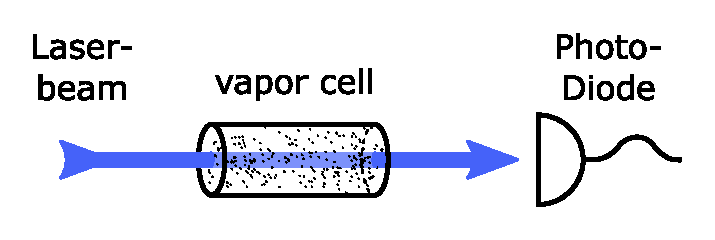
\includegraphics[width=0.35\textwidth]{absorption_spectroscopy_theory}    
    \caption{\label{fig:absorption_spectroscopy} Basic arrangement for ordinary 
        laser absorption spectroscopy.}
\end{wrapfigure}

The arrangement for ordinary laser absorption spectroscopy through a gaseous sample 
is shown in Fig.~\ref{fig:absorption_spectroscopy}. A laser beam passes through 
the vapor cell and its intensity is measured by a photodiode detector as the laser 
frequency \(\nu \) is scanned through the resonance frequency of an atomic transition. \\
To understand the absorption spectroscopy signal we will establish the basic 
equation describing how the laser intensity changes as it propagates through the 
sample. 
\pagebreak

%********************************** % Forth Section  **************************************
\section{Equation} %Section - 2.4
When a laser beam propagates through a gaseous sample only absorption and stimulated
emission change the intensity \(I\) of the laser beam and at the same time affect 
the proportion of the atoms in the ground \(P_0\) and exited state \(P_1\). 
Therefore the intensity at \(x+\dd x\) equals the intensity at \(x\) reduced by 
the missing intensity due to absorption and increased by the intensity due to 
stimulated emission. Each time there is an absorption process the atom absorbs 
the energy \(h\nu \) from the beam. The rate of absorption is defined by 
\(\alpha I \), so the power dissipated by one atom is \(\alpha I \cdot h\nu \). The number \(N\) of interacting
atoms with the beam is the atom density \(n_0\) multiplied by the considered volume
\(V = A \cdot \dd x \) where A is the beam cross section. Only the proportion of atoms in the 
ground state can contribute to the decrease in intensity, so the dissipated power
by absorption is
\begin{align}
    \alpha~I(x) ~ h\nu ~ n_0 ~ A ~ \dd x ~ P_0 ~ 
\end{align}
where \(P_0\) is the proportion of atoms in the ground state.
With the definition of \( intensity = \frac{power}{area}\) one obtains the dissipated
intensity by absorption 
\begin{align}
    \alpha~I(x) ~ h\nu ~ n_0 ~ P_0 ~ \dd x ~. 
\end{align}
Similarly for the stimulated emission the produced intensity is
\begin{align}
    \alpha~I(x) ~ h\nu ~ n_0 ~ P_1 ~ \dd x ~, 
\end{align}
where \(P_1\) is the proportion of atoms in the excited state and \(P_0+P_1 = 1\).
The variation of the laser intensity from \(x\) to
\(x+\dd x\) in the sample is as follows:
\begin{align} \label{eq:Int}
    I(x+\mathrm{d}x)-I(x) = - \alpha~I(x) ~ h\nu ~ n_0 ~ (P_0-P_1)~\mathrm{d}x 
\end{align}
This leads to the differential equation
\begin{align}\label{eq:diff_eq}
    \frac{ \mathrm{d}I }{ \mathrm{d}x } = -\kappa ~ I
\end{align}
where the \textit{absorption coefficient} (fractional absorption per unit of length)
\begin{align}\label{eq:kappa}
    \kappa = \alpha ~ h\nu  ~ n_0 ~ (P_0-P_1)
\end{align}

It should be noted that the proportionality to \(P_0-P_1 \) arises from the 
competition between stimulated emission and absorption and it is important to 
appreciate the consequences. If there are equal numbers of atoms in the ground 
and excited state (\(P_0-P_1=0\)), laser photons are as likely to be emitted by 
an atom in the excited state as they are to be absorbed by an atom in the ground 
state and there will be no attenuation of the incident beam. The attenuation 
maximizes when all atoms are in the ground state (\(P_0-P_1=1\)) because only 
absorption is possible. And the attenuation can even reverse sign (become an 
amplification as it does in laser gain media) if there are more atoms in the 
excited state (\(P_0>P_1\)).

%********************************** % Fifth Section  *************************************
\section{Doppler shifts}  %Section - 2.5

Atoms in a vapor cell move randomly in all three directions with a velocity 
distribution dependent on the temperature. Only the component of velocity parallel 
to the laser beam direction will be important when taking into account Doppler 
shifts and it is this component we refer to with the symbol \(v \). The density 
of atoms \(\dd n \) in having a velocity comprised between \(v \) and \(v+\dd v \) 
is given by the Boltzmann velocity distribution:
\begin{align}
    \dd n = n_0 ~ \sqrt{ \frac{m}{2\pi~k_B T} }~
    \exp{ \left( -\frac{m~v^2}{2~k_B T} \right ) }~\dd v
\end{align}
defining the standard deviation
\begin{align}
    \sigma_v = \sqrt{\frac{k_B T}{m}}
\end{align}
It can be rewritten using the canonical form of a Gaussian distribution
\begin{align}
    \dd n = n_0~\frac{1}{\sqrt{2\pi}~\sigma_v}~
    \exp{ \left( -\frac{v^2}{2~{\sigma_v}^2} \right ) }~\dd v
\end{align}
with a mean of zero~--~indicating the atoms are equally likely to be going in the
positive or negative \(z \) direction, i.e.\ they have positive or negative 
velocities. It is properly normalized so that the integral over all velocities 
(\(-\infty \rightarrow \infty) \) is \(n_0 \), the overall atom density. \\
Atoms moving with a velocity \(v \) see the laser beam Doppler shifted by the 
amount \(\nu~\frac{v}{c} \). This corresponds to a Doppler shifted resonance frequency
\begin{align}\label{eq:nu_shift}
    \nu'_0 = \nu_0 \left ( 1 + \frac{v}{c} \right)
\end{align}
in the lab frame. The sign has been chosen for a laser beam propagating in the 
positive direction so that the resonance frequency is blue shifted to higher 
frequencies if \(v \) is positive and red shifted if \(v \) is negative.\\
The absorption coefficient \(\dd\kappa \) from a velocity group \(\dd n \) at a 
laser frequency \(\nu \) is then obtained from Eq.~\ref{eq:kappa} by substituting 
\(\dd n \) for \(n_0 \) and by adjusting the Lorentzian dependence of \(\alpha \) 
so that it is centered on the Doppler shifted resonance frequency \(\nu'_0 \) 
(Eq.~\ref{eq:nu_shift}).
\begin{align}
    \dd\kappa = \alpha_0 ~ h\nu ~ (P_0-P_1) ~ \mathcal{L}(\nu,\nu'_0)~\dd n
\end{align}
The absorption coefficient from all atoms is then found by integrating over all 
velocity classes.

%********************************** % Sixth Section  *************************************
\section{\label{sec:weakfield}Absorption coefficient~-~weak field}   %Section - 2.6

We consider the weak-laser intensity case, where we have a very low intensity compared to 
\(I_\mathrm{s}\) and therefore nearly all atoms will be in the ground state, i.e., 
\(P_0-P_1 = 1 \) so that
\begin{align}
    \mathrm{d}\kappa = \alpha_0 ~ h\nu ~ n_0~\frac{1}{\sqrt{2\pi}~\sigma_v} ~
    \mathcal{L}(\nu,\nu'_0)~\exp{ \left( -\frac{v^2}{2 {\sigma_v}^2} \right ) }~
    \dd v
\end{align}
and
\begin{align}
    \kappa = \underbrace{ \alpha_0 ~ h\nu ~ n_0 ~ \frac{1}{\sqrt{2\pi}\sigma_v} }_{\beta} 
    \int\limits_{-\infty}^{\infty} 
    \frac{1}{ 1+4~{\left [\nu-\nu_0\left ( 1 + \frac{v}{c} \right) \right] }^2 / {\Gamma_\nu}^2 }~ 
    \exp{ \left (-\frac{v^2}{ 2~ {\sigma_v}^2 }\right ) }~\dd v
\end{align}
After the variable transformation
\begin{align*}
\left |~
    \begin{aligned}
        \nu'_0 =&~\nu_0\left ( 1+ \frac{v}{c} \right) \\
        v =&\left ( \frac{\nu'_0}{\nu_0} - 1 \right) c \\
        \dd v =&~\frac{c}{\nu_0}~\dd \nu'_0
    \end{aligned}
    ~\right |~ = \beta~\frac{c}{\nu_0} \int\limits_{-\infty}^{\infty} 
    \frac{1}{ 1+4~{(\nu-\nu'_0)}^2 / {\Gamma_\nu}^2 }~ 
    \exp{ \left ( -\frac{{(\nu'_0 - \nu_0)}^2~c^2 }{2~{\nu_0}^2~{\sigma_v}^2 } \right )}~
    \dd \nu'_0
\end{align*} 

and substitution \(\sigma_\nu = \frac{\nu_0}{c}~\sigma_v \) we get
\begin{align}
    \kappa = \beta~\frac{c}{\nu_0} \int\limits_{-\infty}^{\infty} 
    \frac{1}{ 1+4~{(\nu-\nu'_0)}^2 / {\Gamma_\nu}^2 }~ 
\exp{ \left ( -\frac{{(\nu'_0 - \nu_0)}^2 }{2~{\sigma_\nu}^2 } \right )}~\dd \nu'_0 
\label{eq:intlorgau}
\end{align}
Now we compare the width parameters from the Lorentzian (see table~\ref{table:iso_prop}) 
with the Gaussian function and at room temperature (\SI{20}{\degreeCelsius}) (see
Fig.~\ref{fig:gauvslor}):

\begin{minipage}[c][][c]{.45\textwidth}
\centering
\begin{align*}
    &\sigma_\nu = \frac{c}{\lambda_\mathrm{D2}}~\sqrt{\frac{k_B T}{m_{Rb85}~c^2}} 
    \approx \SI{403}{\mega\hertz} \\ \\
    &\Gamma_{\nu,\mathrm{D2}} = \SI{0.282}{\mega\hertz} \\ \\
    &\Rightarrow \Gamma_{\nu,\mathrm{D2}} \ll \sigma_\nu
\end{align*}
\end{minipage}
\hfill
\begin{minipage}[c]{.45\textwidth}
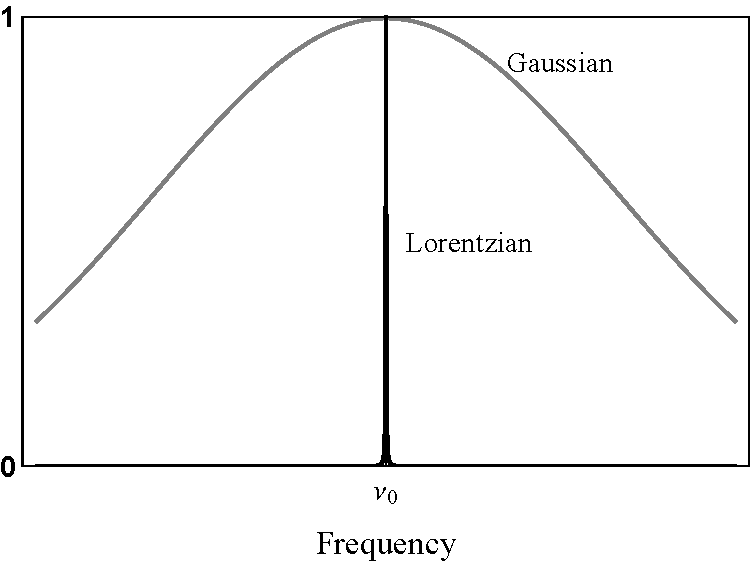
\includegraphics[width=\textwidth]{gauvslor}
\captionof{figure}{\label{fig:gauvslor} The Lorentzian compared to the Gaussian profile}
\end{minipage}
\bigskip

As we can see the Lorentzian function is significantly different from zero only 
within a very narrow range. Consequently the Gaussian remains relatively constant 
over the width of \(\Gamma_{\nu,\mathrm{D2}} \). Therefore Eq.~(\ref{eq:intlorgau}) 
can be accurately determined as the integral of the Lorentzian times the 
value of the exponential at \(\nu'_0 = \nu \):
\begin{align}
    = \beta~\frac{c}{\nu_0}~
    \exp{ \left ( -\frac{{(\nu - \nu_0)}^2 }{2~{\sigma_\nu}^2 } \right )} 
    \int\limits_{-\infty}^{\infty} \frac{1}{ 1+4~{(\nu-\nu'_0)}^2 / {\Gamma_\nu}^2 }~
    \dd \nu'_0
\end{align}
and with the solution of the Lorentzian integral
\begin{align}
    \int\limits_{-\infty}^{\infty} \mathcal{L}(\nu,\nu'_0)~\dd \nu'_0 = 
    \frac{\pi~\Gamma_\nu}{2}
\end{align}
we finally get the absorption coefficient in a weak field
\begin{align}\label{eq:kappa_weakfield}
    \kappa = \kappa_0~\exp{ \left ( -\frac{{(\nu - \nu_0)}^2 }{2~{\sigma_\nu}^2 } \right )}
     ~~\text{with}~~ \kappa_0 = \alpha_0 ~ h\nu ~ n_0 ~ \frac{1}{\sqrt{2\pi}~\sigma_\nu}~
     \frac{\pi~\Gamma_\nu}{2}
\end{align}


%********************************** % Seventh Section  *************************************
\section{Population}   %Section - 2.7

To determine the general case of the absorption coefficient we need to determine 
\(P_0-P_1 \). For that we have to take into account the changes to the ground and 
excited state populations arising from a laser beam propagating through the cell. 
The rate equations for the ground and excited state are therefore:
\begin{align}
    \frac{\mathrm{d}P_0}{\mathrm{d}t} &= \Gamma_{\omega,tot} P_1 - \alpha~I (P_0-P_1) \nonumber \\
    \frac{\mathrm{d}P_1}{\mathrm{d}t} &= -\Gamma_{\omega,tot} P_1 + \alpha~I (P_0-P_1)
\end{align} 
where the first term on the right in each equation arises from spontaneous emission 
and the second term arises from absorption and stimulated emission.\\
With the additional equation \(P_0+P_1=1 \) and the steady state condition
\begin{align}
    \frac{\mathrm{d}P_0}{\mathrm{d}t} = \frac{\mathrm{d}P_1}{\mathrm{d}t} = 0
\end{align}
we get for the populations
\begin{align}
        P_0 = \frac{\Gamma_{\omega,tot} + \alpha~I}{\Gamma_{\omega,tot} + 2 \alpha~I}~; 
        \qquad 
        P_1 = \frac{\alpha~I}{\Gamma_{\omega,tot} + 2 \alpha~I}
\end{align}
which leads to
\begin{align}
    (P_0-P_1) = \frac{\Gamma_{\omega,tot}}{\Gamma_{\omega,tot} + 2 \alpha~I} 
\end{align}
As we can see the population difference is dependent on \(\Gamma_{\omega,tot} \) 
(spontaneous decay rate), which is related to the \textit{Lorentzian width parameter}. 
To combine the Lorentzians in \(\alpha \) (Eq.~\ref{eq:alpha}) and \( (P_0-P_1) \) 
we will define \(\Delta\nu = 2~(\nu-\nu_0) \):
\begin{align}
    \alpha = \alpha_0~\frac{1}{ 1+ \Delta\nu^2 / {\Gamma_\nu}^2 } 
    = \alpha_0~\frac{\Gamma_\nu^2}{\Gamma_\nu^2 + \Delta\nu^2}~; \qquad
    (P_0-P_1) = \frac{2\pi~\Gamma_{\nu,tot}}{2\pi~\Gamma_{\nu,tot} + 2 \alpha~I}
\end{align}
and get
\begin{align}
    (P_0-P_1)\alpha = \frac{2\pi~\Gamma_{\nu,tot}}
    {2\pi~\Gamma_{\nu,tot} + 2I~\alpha_0~\frac{\Gamma_\nu^2}{\Gamma_\nu^2 + \Delta\nu^2}}~ 
    \alpha_0~\frac{\Gamma_\nu^2}{\Gamma_\nu^2 + \Delta\nu^2} = 
    \frac{\alpha_0~\pi~\Gamma_\nu^2~\Gamma_{\nu,tot}}
    {\pi~\Gamma_{\nu,tot}~(\Gamma_\nu^2 + \Delta\nu^2)+I~\alpha_0~\Gamma_\nu^2}
\end{align}
dividing with \(\pi~\Gamma_\nu \) and substitute in the denominator \(\alpha_0 \) 
with the definition of Eq.~\eqref{eq:gamma_relation} and~\eqref{eq:saturationInt} 
leads to
\begin{align}
    (P_0-P_1)\alpha = \alpha_0~\frac{1}
    {1 + \frac{\Delta\nu^2}{\Gamma_\nu} + \frac{2I}{I_s}\frac{\Gamma_\nu}{\Gamma_{\nu,tot}} } 
    = \frac{\alpha_0}{(1 + \frac{2I}{I_s}\frac{\Gamma_\nu}{\Gamma_{\nu,tot}})}~
    \frac{1}{1+ \frac{\Delta\nu^2}
    {\Gamma_\nu^2 \left(1 + \frac{2I}{I_s}~\frac{\Gamma_\nu}{\Gamma_{\nu,tot}} \right)}}
\end{align}
and with the definition of the power-broadened \textit{width parameter}
\begin{align}
    \Gamma'_\nu = \Gamma_\nu \sqrt{1 + \frac{2I}{I_s}~\frac{\Gamma_\nu}{\Gamma_{\nu,tot}} }
\end{align}
we obtain
\begin{align}\label{eq:kappa_weak}
    (P_0-P_1)\alpha = 
    \frac{\alpha_0}{ \left( 1 + \frac{2I}{I_s}\frac{\Gamma_\nu}{\Gamma_{\nu,tot}} \right )}~
    \mathcal{L}'(\nu,\nu_0)~~\text{and}~~\mathcal{L}'(\nu,\nu_0)= 
    \frac{1}{1+ \frac{{4~(\nu-\nu_0)}^2}{{\Gamma'_\nu}^2}}
\end{align}

%********************************** % Eighth Section  *************************************
\section{Absorption coefficient~-~general case}  %Section - 2.8

For the general case we take now into account the velocity groups and their 
corresponding Doppler shifts for the case \(P_0-P_1 \neq 1 \) and therefore 

\begin{align}
    \mathrm{d}\kappa = 
    h\nu~n_0~\frac{\alpha_0}{(1 + \frac{2I}{I_s}~\frac{\Gamma_\nu}{\Gamma_{\nu,tot}})} 
    \frac{1}{\sqrt{2\pi}~\sigma_v} \mathcal{L}'(\nu,\nu'_0) 
    \exp{ \left( -\frac{v^2}{2~{\sigma_v}^2} \right ) } \dd v
\end{align}
and
\begin{align}
    \kappa = h\nu~n_0~\frac{\alpha_0}{(1 + \frac{2I}{I_s}~\frac{\Gamma_\nu}{\Gamma_{\nu,tot}})}~ 
    \frac{1}{\sqrt{2\pi}~\sigma_v} 
    \int\limits_{-\infty}^{\infty} 
    \frac{1}{ 1+4~{\left [\nu-\nu_0\left ( 1 + \frac{v}{c} \right) \right] }^2 / {\Gamma'_\nu}^2 } 
    \exp{ \left (-\frac{v^2}{ 2~{\sigma_v}^2 }\right ) } \dd v
\end{align}
The calculation can be performed as in Section~\ref{sec:weakfield} with the only 
addition of the the power-broadened \textit{width parameter} \(\Gamma'_\nu \). 
This leads to
\begin{align}
    \kappa &= h\nu~n_0~
    \frac{\alpha_0}{(1 + \frac{2I}{I_s}~\frac{\Gamma_\nu}{\Gamma_{\nu,tot}})}~ 
    \frac{1}{\sqrt{2\pi}~\sigma_\nu}~\frac{\pi~\Gamma'_\nu}{2}~
    \exp{ \left ( -\frac{{(\nu - \nu_0)}^2 }{2~{\sigma_\nu}^2 } \right )} \nonumber \\
    &= \frac{\kappa_0}{\sqrt{1 + \frac{2I}{I_s}~\frac{\Gamma_\nu}{\Gamma_{\nu,tot}}}}~
    \exp{ \left ( -\frac{{(\nu - \nu_0)}^2 }{2~{\sigma_\nu}^2 } \right )}
\end{align}
and subsequently
\begin{align}
    \kappa = \kappa'_0~\exp{ \left ( -\frac{{(\nu - \nu_0)}^2 }{2~{\sigma_\nu}^2 } \right )}
    ~~\text{with}~~ \kappa'_0 = 
    \frac{\kappa_0}{\sqrt{1 + \frac{2I}{I_s}~\frac{\Gamma_\nu}{\Gamma_{\nu,tot}}}}~.
    \label{eq:kappa_final}
\end{align}


%********************************** % Ninth Section  *************************************
\section{Beer-Lambert Law}  %Section - 2.9
As derived before (Eq.~\ref{eq:kappa_final}) \(\kappa \) is dependent on the 
intensity, so solving Equation~\ref{eq:diff_eq} is not an easy task. But in the 
case of low intensity we can make an assumption that \(\kappa \) is independent
from \(I\). The solution of the differential equation is then:
\begin{align}\label{eq:beer_lambert}
   I(x)=I_0~\mathrm{e}^{-\kappa x}~.
\end{align}
This solution is called \textit{Beer-Lambert law} and will be used in Chapter 4 
as basis for our evaluation.
\pagebreak


%********************************** % Tenth Section  *************************************
\section{Real Rb atom D2 line levelscheme}\label{sec:realrubidium} %Section - 2.10

\begin{figure}[ht]
    \centering
    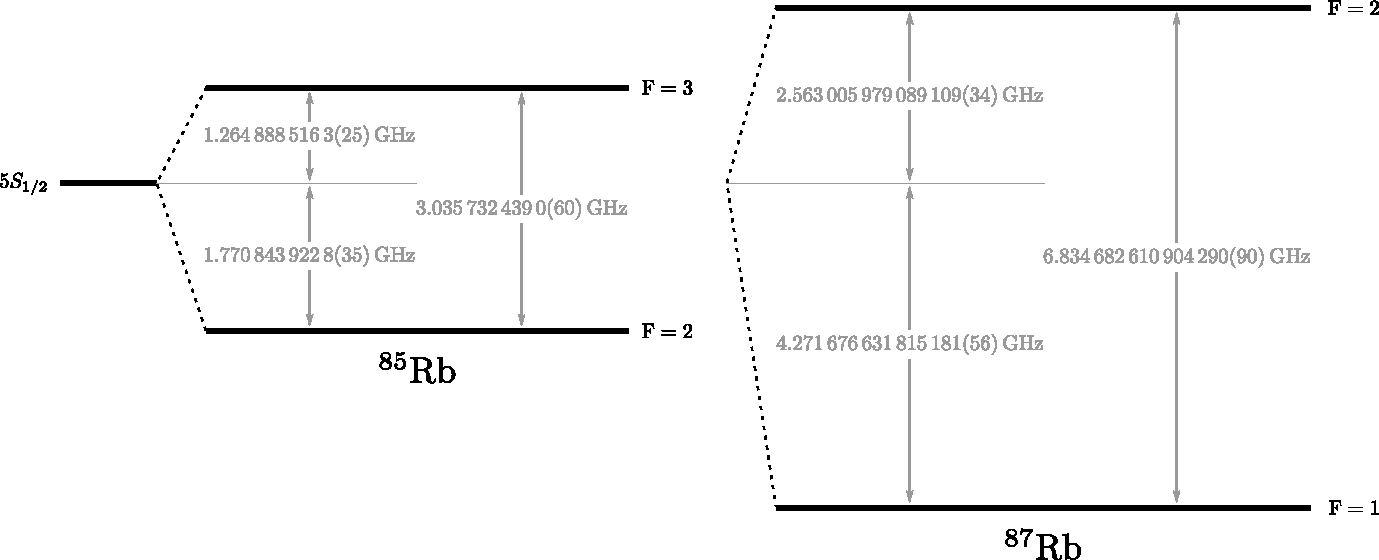
\includegraphics[width=0.95\textwidth]{hyperfine_scheme}
    \caption{\(5^{2}S_{1/2} \) hyperfine structure of \(^{85}\)Rb 
    and \(^{87}\)Rb.}    
\end{figure}

The transition of interest is, as we have discussed before, the \(5^{2}S_{1/2} 
\rightarrow 6^{2}P_{3/2}\) of rubidium. In the cell we use, two isotopes of Rb 
are present: \(^{85}\)Rb and \(^{87}\)Rb.
As we can see both isotopes have the same transition energy, but due to the 
different spin I (see table:~\ref{table:iso_prop}) the hyperfine energy splitting
is different \citep{nist_asd}: \SI{3}{\giga\hertz} for \(^{85}\)Rb and 
\SI{6.8}{\giga\hertz} for \(^{87}\)Rb. This is the reason why we witness four 
Doppler peaks in our spectrum when performing a spectroscopy (see Fig.~\ref{fig:doppler}). 
The different amplitudes between the two isotopes are explained through their 
abundance in the cell, \SI{72.2}{\percent} for \(^{85}\)Rb and \SI{27.8}{\percent} 
for \(^{87}\)Rb. And the cause for the difference among one isotope is that the 
different hyperfine states, e.g.~\(F=2\) and \(F=3\) for \(^{85}\)Rb, have 
\(m_F = 2F+1 \) distinct levels. The thermal energy at \SI{300}{\kelvin} is 
three orders in magnitude higher than the hyperfine splitting and thus each of 
the \(m_F\) levels are equally populated.  

\begin{figure}[h]
\centering
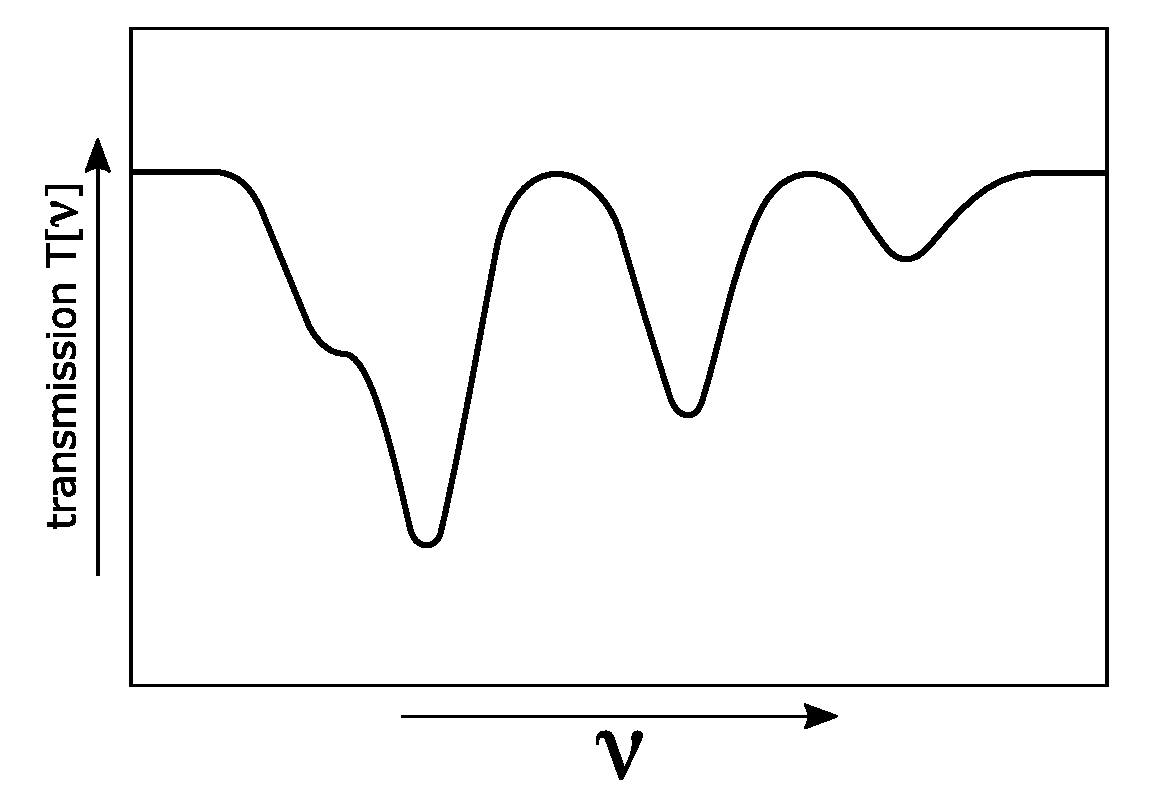
\includegraphics[width=0.5\textwidth]{spectrum_doppler}
\caption{\label{fig:doppler}Doppler spectrum of D2 line} 
\end{figure}

\pagebreak
%********************************** % Eleventh Section  **********************************
\section{Rubidium data}  %Section - 2.11

\begin{table}[h]
\centering
\begin{tabular*}{0.9\textwidth}{@{\extracolsep{\fill} }l l c c}
\toprule
& & \multicolumn{2}{c}{Rubidium} \\
\midrule
Isotope & [1] & 85 & 87 \\
Atomic mass & [\si{\atomicmassunit}] & 84.911794 & 86.909187 \\
\num{e-25} & [\si{\kilogram}] & 1.40999 & 1.44316 \\
Abundance & [\si{\percent}] & 72.17 & 27.83 \\
Spin I & [1] & \(\sfrac{5}{2}\) & \(\sfrac{3}{2}\) \\
Lifetime \(6^{2}P_{3/2}\) & \([ \si{\nano\second} ]\) & & \num{112} \\
Lifetime \(6^{2}P_{1/2}\) & \([ \si{\nano\second} ]\) & & \num{125} \\
Wavelength D1-Line (\(6^{2}P_{1/2} \rightarrow 5^{2}S_{1/2}\)) & [\si{\nano\meter}] & 421.5524 & \\
Wavelength D2-Line (\(6^{2}P_{3/2} \rightarrow 5^{2}S_{1/2}\)) & [\si{\nano\meter}] & 420.1792 & \\
A\(_{\mathrm{ki,D1}},~\Gamma_{\omega,\mathrm{D1}}\) @ \SI{421}{\nano\meter} & \([ \si{\per\second} ] \) & \num{1.50e6} & \\
A\(_{\mathrm{ki,D2}},~\Gamma_{\omega,\mathrm{D2}}\) @ \SI{420}{\nano\meter} & \([ \si{\per\second} ] \) & \num{1.77e6} & \\
Natural linewidth \(\Gamma_{\nu,\mathrm{D1}}\) & \([ \si{\mega\hertz} ]\) & \num{0.239} & \\
Natural linewidth \(\Gamma_{\nu,\mathrm{D2}}\) & \([ \si{\mega\hertz} ]\) & \num{0.282} & \\
\bottomrule
\end{tabular*}
\caption{\label{table:iso_prop}Properties of rubidium isotopes}
\end{table}
\pagebreak


